\chapter{Towards reproducible, open science through open research software}
\section{Introduction}


% FIXME: Deleted
% Science: giants, collective, grows when shared
% Web: money, open-source, tools esp. DVCS
% Computing: performance, GPU
% Changes: dynamics, way science is done, coding inferior, open science

% see http://sciencecodemanifesto.org/
% http://lorenabarba.com/gallery/reproducibility-pi-manifesto/
% https://www.numfocus.org/
%
% http://www.nature.com/news/interactive-notebooks-sharing-the-code-1.16261
% We provide examples of solutions for: Good coding practice, source control
% management, packaging, licenses documentation, testing,CI

% Fluiddyn: foster open-science, source. Framework for collaborative dev, open
% methods

In order to attain the research goals in this thesis, a path off the beaten
track was pursued -- i.e. to create a handful of easy to maintain, rigorously
tested, and most-importantly, open-source scientific packages which do not
compromise on performance.
%
This resulted in the creation of FluidDyn, a project to facilitate open-science
in the field of fluid mechanics.
%
The focus of the project was to develop a set of packages to implement a
framework for simulations \citep{fluidsim}, experiments
\citep{augier_fluidimage_2016,augier_fluidlab_nodate}, Fast Fourier Transforms
\citep{fluidfft} -- all depending on a base package to reuse certain utilities
and data structures \citep{fluiddyn}.
%
The project owes a lot to the recent developments in methods and tools for
open-source software engineering.
%
Several modern coding practices were adopted while developing these packages.


The FluidDyn packages are primarily written in Python language. Incidentally,
it is the defining characteristics of Python which make the eventual success of
such a project realizable.
%
Python is one of the most important tools in recent open-source dynamics,
particularly in science.
%
The popularity of the language in fluid mechanics is growing, but Python is yet
to reach widespread adoption as the language of choice. 

We shall now discuss these topics in greater detail. The chapter is organized
into four sections. The first section focusses on the technical aspects, with
particular focus on emerging developments in programming languages, tools and
services suited for open-source software development. The subsequent section
presents Python's strengths and weaknesses as a language for scientific
computing.
%
The third section compares various software development methodologies. Here, we
will also discuss about the possible contradiction between productivity of
individuals and productivity at the community level.
%
The chapter finally ends with a summary of the motivations for the project
FluidDyn and an overview of the packages we have developed.
% The chapter ends with a note on the capabilities of FluidDyn
% packages\footnote{We use FluidDyn (with capital letters) to name the project
% and \fluiddyn for the base package.}.
%

% \section{Science, software, open-source and the computer revolution}
\section{Open-source software and open-science}

Computational sciences, and especially computational fluid dynamics (CFD) as a
discipline, have flourished in the latter half of the twentieth century.
Incidentally, the origin of this discipline can be traced back to the ideas in
\citet{richardson_weather_1922} to achieve numerical weather prediction.
Following the arrival of first electronic general-purpose computer, ENIAC in
1945, the first simulations were made by \citet{charney_numerical_1950} using a
simple barotropic model to make 24 hour forecasts \citep[see
also][]{lynch_richardson_2010}. In those early days when the availability of
computers was limited, such methods were neither widespread nor feasible.
Scientific investigations were dominated by theoretical and experimental
methods.
%
We have come a long way and today computational methods complement theoretical
and experimental studies, and are equally important.
%
% Thus, in a typical scientific study, there is significant effort involved in
% translating the mathematical representation to a working research software.
%
With the connectivity provided by the world wide web it is possible to achieve
more and reinvent the way we do sciences.

\begin{figure}[h]
  \centering
  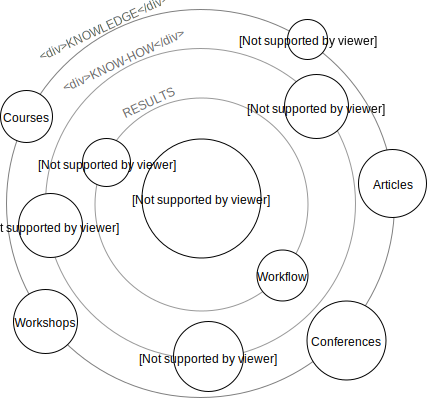
\includegraphics[width=0.8\textwidth]{open_science}
  \caption{A schematic representation of various concepts and methodologies
  involved in achieving reproducibility in sciences.}\label{fig:opensci}
\end{figure}

In recent years, there has been a move towards open science
\citep[see the report by][]{royal_society_great_britain_science_2012}.
%
Depicted in figure~\ref{fig:opensci} are some of steps needed to ensure
reproducibility and transparency in sciences.
%
Traditionally, \emph{knowledge} has been disseminated in the form of courses
and books from universities, and to the wider scientific community through
research articles, conference proceedings and workshops.
%
In the last decade, knowledge has become more accessible to the public
through public-domain and Creative Commons (or similar) licensed course
materials and massively open online courses (MOOCs). Moreover, there is also an
emerging push to publish in open-access journals\footnote{In the European
  Union, a proposal to implement Plan S (\url{https://www.coalition-s.org}) was
  been set in motion in September 2018 to fast track adoption of open-access.
} either through systematic
reforms in academia on how researchers' productivity are assessed, or through
regulations and offering incentives, such as waiving the application processing
charge for publishing \citep{nosek_promoting_2015}.

A lot of work is required to condense and implement this knowledge in the form
of working applications.
%
The \emph{know-how} can be made accessible and open to scrutiny by making
research software open-source with an appropriate license\footnote{For a
	detailed comparison of licenses, visit either
	\url{https://choosealicense.com} or
	\url{https://www.gnu.org/licenses/license-list.html}. }.
%
To make codes usable they have to be complemented by documentation which
typically includes tutorials, examples and a detailed commentary of different
components.
%
Furthermore, to inspire confidence in and to ensure reliability of a code
throughout the process of software development, it needs unit-tests through
which it is continuously built, tested and deployed --- a process known as
Continuous Integration (CI). Depending on how matured a software is, CI can be
easy or cumbersome to implement, but nevertheless, the result is a cleaner and
reliable code.

Finally, the \emph{results} generated from such codes together with the
workflow (i.e.\ scripts to run the codes and to post-process the data) when made
open in the form of datasets can ensure that research is reproducible and
preserved in archives for several years to come \citep{gewin_data_2016}. Open
datasets can be shared and made citable through services such as
\href{https://zenodo.org}{Zenodo} and \href{https://figshare.com}{Figshare}.

In FluidDyn project, we have strived to implement all the aspects of making the
know-how open through open-source software. We shall now take a look at the
tools which have made it possible.

\subsection{Methods and tools for open-source software engineering}

\subsubsection{Free and Open-Source Software}

The Free and Open-Source Software (FOSS) movement has given rise to the tools
that enable open-source software development today.
%
The term \emph{free} in FOSS is a misnomer, as it actually stands for
\emph{freedom} (to use, modify and distribute). The FOSS movement has
dramatically decreased the cost of using computers, which is evident from the
widespread use of GNU/Linux systems in desktops, computing clusters and
web-servers in academia and beyond.
%
The FOSS culture can be traced back to the success of typesetting
standards \TeX\ (1977) and \LaTeX\ (1985) for authoring scientific publications.
%
Another founding moment for the FOSS movement was the launch of the GNU project
in 1983 by \href{https://en.wikipedia.org/wiki/Richard_Stallman}{Richard
  Stallman}, to create a Unix-like computer operating system composed entirely
  of free software\footnote{For completeness, see also the work done on
  \href{https://www.levenez.com/unix/}{other Unix operating systems, for
example BSD}.}.
%
GNU is today known for its compiler collection (GCC) and a multitude of tools
which combined with the Linux kernel (created by
\href{https://en.wikipedia.org/wiki/Linus_Torvalds}{Linus Torvalds} in 1991)
forms the GNU/Linux operating system
% and its several distributions (Debian, Red Hat, Slackware, Arch Linux and
% Gentoo to name a few)
that we are familiar with today.
%
% FOSS movement has had huge successes in many frontiers --- Apache could be
% termed as the ``first killer-app of Linux'' and now with an ever-increasing
% suite of softwares including Firefox, LibreOffice, Gimp as solid alternatives
% to proprietary offerings.
%
Linux has become the most widely used kernel, being deployed on servers,
personal computers, embedded devices, and also smart phones (with Android). The
success of the Linux kernel project was attributed to the \emph{bazaar} model of
software development, as described in \citet{raymond_cathedral_1999}, wherein a
code can stay structured despite releasing frequently and delegating tasks to
community with myriad agendas.

% remark Julien Salort: not interesting. Nothing on BSD.
% https://www.levenez.com/unix/

Over the years, FOSS development has transitioned from an organic community of
volunteers, towards an organized system with participation from industries,
non-profit organizations and government institutions.
%
Such a model results in a win-win scenario -- users benefit from transparency and
ability to tinker, and the organizations profit with more contributions.
%
The FOSS movement has now entered into a second era
\citep{fitzgerald_transformation_2006}.

% - 90s arrival of internet (soon mass market)

% Some huge open-source successes : Apache ("first killer app of Linux"),
% now Firefox, Open-office
% av: https://www.reddit.com/r/AskReddit/comments/7x639l/what_free_software_is_so_good_you_cant_believe/du6pw11/

% Linux kernel now widely used on servers, personal computers, embedded
% devices, smarth phone (with Android).
% https://en.wikipedia.org/wiki/Linux_kernel

% Now, new period for open-source: 
% see http://www.cepis.org/upgrade/files/full-2005-III.pdf

% - "Libre Software Movement: The Next Evolution of The IT Production
% Organization?"

% - ``the composition of development teams was changing, from all-volunteer
% teams to teams with paid participants from industry, government or
% not-for-profit organizations.''

% By the way, we also have to use the term "libre software" (?)
% av: Libre-software is not so mainstream. Even Linux kernel is not libre with
% binary blobs for drivers.

% We may have to change the order of this list?
% - git and mercurial 2005
% - software repositories ~ 10 years before
% so I would exchange the too paragraph...
% av:That is probably because we did not mention patches and CVS, subversion
% etc.

\subsubsection{Source code management}

Collaboration was achieved in the early years of FOSS development through
emailing ``patches'', and centralized Version Control Systems (VCS) near the
turn of the 21\textsuperscript{st} century.  The collective collaboration on
development is today streamlined with the emergence of Distributed Version
Control Systems (DVCS), especially, Git and Mercurial).
%
Version control tools are designed to work on any kind of text files, not just
codes, so they could even be utilized to write scientific documents with
multiple authors.
%
In web-based source development platforms like GitHub, Bitbucket and GitLab,
DVCS repositories are enhanced with code-review tools, typically consisting of
a issue tracker and pull-request mechanism.
%
Git has become the \textit{de facto} standard for source management. However,
for the FluidDyn project, we prefer to use Mercurial because we consider it to
be simpler for the beginners and just as powerful for expert users\footnote{See
  \href{https://www.mercurial-scm.org/wiki/GitConcepts}{``a detailed
comparison''} on Mercurial website.}. Simplicity and low learning barriers for
scientists who are not experts in software development is crucial for our
project.
%
Note that, it is now possible to use Mercurial to work with Git repositories,
for example hosted in GitHub and GitLab\footnote{By using the Mercurial
extension \href{http://hg-git.github.io/}{hg-git}.}.
%
The use of DVCS in science will lead to long term productivity benefits
\citep{wilson_best_2014}.


\subsubsection{Package management and software repositories} 

Packaging process depends on the language used in a project, however some good
practices are universal, such as licensing, supplying documentation (a README
file at the bare minimum), keeping installation paths flexible and relying on
official build tools \citep{taschuk_ten_2017}.
%
A credible repository to packages as compressed archives or as pre-compiled binary
packages is indispensable to promote code reuse and reproducibility of results.
%
The use of repositories started with the conception of
CPAN and CRAN repositories for the languages Perl and R in 1993 --- based on
the Comprehensive \TeX\ Archive Network (CTAN) model for \TeX\ packages. 
%
Python as a medium for scientific computing owes its success to a rich
ecosystem of third-party packages. \href{https://pypi.org}{Python Package
Index (PyPI)} and \href{https://anaconda.org}{Anaconda Cloud} are major
repositories for delivering and downloading Python packages, assisted by
package managers \pack{pip} and \pack{conda} respectively. The
\fnref{https://packaging.python.org}{``Python Packaging User Guide''} is an
excellent guide to learn how to install, package and distribute projects.
% Almost all major
% languages\footnote{\href{https://stackoverflow.com/questions/1693529/%
% list-of-top-repositories-by-programming-language}{https://stackoverflow.com/%
% questions/1693529/list-of-top-repositories-by-programming-language}} have
% similar repositories, with exceptions such as Fortran and Matlab.
Specialized package managers, such as \pack{easybuild} and \pack{spack}, have
also emerged to install scientific libraries and compilers.

\subsubsection{Continuous Integration and documentation} The need for
strong reliability of packages with increasing complexity has forced developers
to use Continuous Integration (CI).
%
When the code depends on a wide variety of external dependencies, CI is useful
to avoid \fnref{https://en.wikipedia.org/wiki/Software\_rot}{software rot},
i.e.\ to avoid obsolescence with newer versions of the compiler or its
dependencies. CI is specifically important for dynamical languages and
open-source code since, it allows open-source projects to welcome contributions
from other developers while maintaining a high degree of reliability.
%
Firstly, the code is \emph{built} against a known, repeatable emulation
environment on a server. Thereafter, a set of \emph{unit tests} are run for
each commit (modification of the code) to check that no bugs have been
introduced. It is also important to analyse what portion of the source code is
covered by these unit tests --- a method referred to as \emph{code coverage}.
%
Almost all CI platforms are free for open-source projects --- Travis CI,
CircleCI and Appveyor to name a few. Bitbucket and GitLab have built-in CI
implementations. Websites such as Codecov and Coveralls help to chart and
analyse the code coverage history, viewable by anyone. To use these services,
one simply has to write a simple file in YAML format and authenticate the
respective services with ``read'' permissions.

New users and developers often rely on good documentation and examples.
Documentation generators such as Sphinx (for Python) and Doxygen (for many
languages including C, C++, Fortran and Python) parses in-line comments into
documentations as PDF, HTML and more \citep{lee_ten_2018}.
%
The documentation generation can be automated online and deployed using any CI.
``Read the Docs'' has, in recent years, become the hub for building and hosting
documentation online, thus facilitating the process for developers and
considerably improving access to information for users.
%
In the FluidDyn project we this limit ourselves to automating tests and
documentation of the latest version. It is possible to further exploit the
CI by adding code style checks by running ``linters'' alongside unit tests,
\emph{continuous delivery} of package releases and preserving older versions of
documentation.

\subsubsection{Knowledge hubs and communication}

% Mutual aid and knowledge sharing have been important aspects of the web since
% its inception and these practices are now of foremost importance for many
% human activities.
%
%In particular, 
Learning programming and computer science is now greatly aided by websites like
the community driven encyclopaedia \href{https://www.wikipedia.org/}{Wikipedia}
or the community driven forum \href{https://stackoverflow.com/}{Stack
Overflow}, where people write thousands of questions and answers on programming
each week. The IRC protocol has continued to sustain the test of time. Instant
messaging channels such as \codeinline{\#python} on Freenode facilitate
interactive discussions and a form of community-level support system --- a role
which used to be filled by mailing lists alone in the past. Alternatives such
as Riot (Matrix protocol), Gitter, and Slack have gained popularity offering
different integration solutions on top of instant messaging.
%
Through instant messaging a geographically separated team, as in the case of
the FluidDyn project, can achieve near real-time collaboration without having
to arrange video conferences or meetings.

Thus, there is a number of new methods and tools in software development.
Taken all together, they greatly improve our collective efficiency and
open possibilities for interactions that were unthinkable a few years ago.
%
For example, the success of community-driven software like \pack{astropy} (a
subject-area research library with
\href{https://github.com/astropy/astropy}{more than 240 contributors}) and
\pack{scikit-learn} (a machine learning toolkit with
\href{https://github.com/scikit-learn/scikit-learn}{more than 1000
contributors}) would not have been possible without these new software
development methods.
%
As scientists, we can wonder how to fully exploit these new possibilities to do
science. The project FluidDyn is an attempt to advance the fluid dynamics
community in this direction.


\section{Python, a programming language adapted for open-science}

We now turn to the presentation of the
\href{https://www.python.org/}{programming language Python}, another
fundamental tool for the FluidDyn project. Note that, this is not a detailed
technical presentation: we focus on the ideas necessary to understand why the
FluidDyn project is based on this language and on facts interesting for
potential FluidDyn users and developers.

The Python community has thrived remarkably in the last few years, which is
evident from the fact that by the end of 2017, Python became the second most
popular language in terms of pull-requests in GitHub\footnote{%
%See GitHub's annual report titled \href
\url{https://octoverse.github.com/2017}
% { ``The State of the Octoverse 2017''}.
%
} and
\fnref%
% [See the blog post ``The Incredible Growth of Python'']%
{https://stackoverflow.blog/2017/09/06/incredible-growth-python/}%
{questions on StackOverflow}.
%
TIOBE-index\footnote{\url{https://www.tiobe.com/tiobe-index}}, which assess the
popularity of a language based on number of skilled users, courses and
third-party vendors, ranks Python at number four. IEEE Spectrum\footnote{
%See the analysis titled 
\url{https://spectrum.ieee.org/computing/software/the-2017-top-programming-languages}
%{``The 2017 Top Programming Languages''} on IEEE spectrum.
}
ranks Python as the most popular language in 2017 with a metric
based on trends, demand by employers and users on open-source hubs.  All the
rankings agree that Python usage has been steadily growing and is here to stay.
Python largely outclasses languages like Fortran and Matlab according to these
statistics, and is now clearly one of the mainstream languages with C, Java,
C++ and JavaScript.
%
The language has been designed to boost the communication of technical ideas
between humans. 
%
Let us summarize some characteristics of the Python languages that have lead to
such an incredible success.
%
Python differs from other mainstream languages for a variety of reasons:


\begin{itemize}
\item \textbf{Aesthetics.} The syntax is expressive, with an inherent emphasis
on readability. Blocks of code are defined with the indentation.

\item \textbf{Code style.} There are official (but, optional) guidelines, named
\fnref{https://www.python.org/dev/peps/pep-0008/}{PEP~8}, advocating for
regularity of the code. Linters and code-formatters can evaluate and enforce
adherence to this style.

\item \textbf{Automatic memory management.}  A garbage collector handles the
memory allocation and deallocation, which needs no user intervention. There
are, of course, ways to control the memory usage of a program, though not as
precisely as for low-level languages.

\item \textbf{Dynamic typing.}
The types of objects are inferred at run time from the code and the
context, and in many situations, one does not need to declare them explicitly.

\item \textbf{Interpreted.} The standard way\footnote{There are also tools to
compile Python code (for example Cython and Pythran).} to run a Python code is
to ``interpret'' it.  A program called the interpreter executes the code
nearly\footnote{Actually, the execution of Python code is less simple and
involves an Abstract Syntax Tree.} instruction-by-instruction, with very few
optimizations.
%
In contrast to other compiled languages, such as Fortran, C or C++, there is no
proper compilation step: the code is not translated to optimized machine
instructions, but only to Python bytecode.

\item \textbf{Multi-paradigm.} Imperative, object-oriented, functional
and aspect-oriented programming are supported.

\item \textbf{Extensible}. It is easy to interface with code written in
several other languages (in particular C, C++ and Fortran).

\item \textbf{Batteries included.} Python comes with a large
\fnref{https://docs.python.org/3/library/index.html}{standard library}.

\item \textbf{Cross platform.} Python can be deployed on many different
machines with different operating systems (Linux, Windows, macOS, Android) and
architectures (from a microcontroller --- with MicroPython or CircuitPython ---
to a Blue Gene supercomputer).

\end{itemize}
%
Thus, Python is one of the best ``glue'' languages for fast prototyping.
Code development in Python is much faster and easier than with many other
languages. Less bugs are introduced by the developers simply because there are
fewer lines of code \citep{nanz_comparative_2015}.
%
Maintaining and modifying existing code is also facilitated by the very good code
readability associated with the language.
%
Another consequence of the apparent simplicity of Python is that the learning
curve has a nice shape. Learning Python is very easy from the start and the
complexity gradually increases as the level of the developer increases.
%
Its interpreted nature is advantageous for a rapid development cycle and the
possibility of interactive workflow (usually with IPython or Jupyter
notebooks).
%
Therefore, Python is good for developers at all levels: very gentle for
beginners and very powerful for advanced users.

Python is an old language (first implementation in 1991!) but it continues to
evolve.
%
Note that there are many implementations of Python
interpreters\footnote{Notable ones are CPython (written in C), Jython (Java),
IronPython (C\#), PyPy (Rpython, a subset of Python) and
MicroPython/CircuitPython (C, targeted to micro-controllers).}. The default and
most widely used implementation is written in C and is called CPython.
%
A hard and controversial decision was taken to clean up Python from its
historical incoherences by introducing a new series of backwards-incompatible
versions of the language, starting with Python 3.0, released in December 2008.
After a long and difficult process, the transition from Python 2 to Python 3 is
completed for nearly all important packages\footnote{Close to
\href{https://python3wos.appspot.com/}{95\% of the most downloaded packages}
are Python 3 compatible as of 2018.}. Especially for scientific applications,
we can now work only in Python 3. For instance, \href{https://github.com/%
numpy/numpy/blob/master/doc/neps/dropping-python2.7-proposal.rst}{future
versions of \Numpy} and \fnref{http://www.python3statement.org/}{the main
scientific packages} will not be compatible with Python 2. These changes
open doors to a very clean, coherent and potentially faster Python
experience. Therefore, one should not use Python 2 for science any more and
instead, adopt the newer versions.
%
New versions of Python have nice features to adapt to new usages and to
recent trends in computer science.  For example, three new features were
introduced in Python 3.5 (first released on September 2015): the \codeinline{@}
operator for matrix multiplication, the new \codeinline{async} and
\codeinline{await} keywords for concurrency and type hinting\footnote{See also our
paragraph on the issue of type checking in the following.} (with the module
\codeinline{typing} and an associated syntax presented in the
\href{https://www.python.org/dev/peps/pep-0484/}{PEP~484}).

Being a very versatile language, Python is widely used for many different
applications\footnote{\href{https://www.jetbrains.com/research/devecosystem-2018/python/}{See
\emph{The State of Developer Ecosystem Survey in 2018} by JetBrains}}:

\begin{itemize}
\item Simple scripting

\item Web development

\item Data science

\item System, database and network administration

\item GNU/Linux distribution software

\item GUI desktop applications

\item Scripting layer for applications (for example Paraview, Visit, QGIS,
	Blender)

\item Web scraping

\item Animation, gaming and film industry

\item Education

\item Science

\end{itemize}
%
Python
% has recently become one of the most popular language for teaching programming
% and developing scientific applications. It 
has now a mature and powerful scientific ecosystem with well-established
foundational packages
%
(\Numpy for N-dimensional homogeneous arrays, \Scipy as the
fundamental toolkit for scientific computing, \pack{Matplotlib} for plotting
and \pack{Pandas} for data structures) and several more specialized packages
(to name a few, \pack{h5py}, \pack{mpi4py}, \pack{skimage}, \pack{sklearn}).
The \href{https://github.com/rougier/python-visualization-landscape}{%
landscape of visualization tools usable through Python} makes it possible to
integrate post-processing and analysis capabilities into a single application.
%
Python is one of the main languages for data science with packages such as
\pack{Pandas}, \pack{statmodels}, \pack{sklearn}, \pack{Keras},
\pack{TensorFlow} and \pack{PyTorch}.
%
There are user-friendly and ready-to-use Python installers (similar to Matlab), in
particular the
\href{https://en.wikipedia.org/wiki/Anaconda_(Python_distribution)}{%
open-source distribution Anaconda} to streamline the installation in 
desktop platforms.
Integrated development environments (IDE) adapted for
scientists, for example \href{https://github.com/spyder-ide/spyder}{Spyder},
\href{https://pyzo.org}{Pyzo},
and \href{https://jupyterlab.readthedocs.io}{JupyterLab} are often useful for
interactive development.

Python has a very large and supportive community (see, for example,
\fnref{http://stackoverflow.com/tags/python}{Stack Overflow tags}).
%
Python development is also supported by companies, and most of them specialize
in web technologies and data-driven research. However, recently, companies
involved in scientific software development have started to become quite
influential. For example, Anaconda Inc.\ is strongly engaged in the development
of tools like JIT Python accelerator \pack{Numba}, and parallelism framework
\pack{dask}. Hardware giants such as Intel and Nvidia also contribute to the
Python scientific ecosystem.
%
To summarize, Python's numerous features and its adoption in several domains
makes it a sensible language choice for scientific purposes.

\subsection{Some Python issues and their solutions}

In the context of scientific computing there are some common issues that Python
developers would face. The issues are listed below and the solutions are
specified briefly. The solutions are explained in further detail in subsequent
paragraphs.

\begin{itemize}

\item \textbf{Performance in CPU bounded tasks.} Since the standard Python
	interpreter does not do any proper compilation, pure Python code for
	some CPU bounded tasks can be too slow. Thus, one has to avoid writing
	loops as much as possible and use vectorized array operations as much
	as possible. One can also call \emph{foreign functions}, or use special
	tools to build extensions using \emph{Ahead Of Time} or \emph{Just In
	Time} compilation to speedup performance-critical code.

\item \textbf{Absence of type checking.} In contrast to compiled languages,
	there is no type-checking in Python (and more generally in many
	interpreted languages). Types are respected however, and type errors,
	if any, would be raised during runtime.
	\emph{Type hints} and \emph{static type checking} can solve this issue.

\item \textbf{Concurrent, but not parallel multi-threading.} Threads behave
	like light sub-programs. In principle, they can use the different cores
	of the CPU at the same time, but the CPython interpreter forbid threads
	to interpret python code at the same time\footnote{See
	\url{https://opensource.com/article/17/4/grok-gil}
	%{a blog article ``How to grok the GIL''}
	% and \url{https://faster-cpython.readthedocs.io/cpython37.html}{a
	% technical presentation by a CPython core developer}.
	}. In other words, threads can coexist concurrently, by not executing in
	parallel.
%
This limitation comes from an important detail in the implementation of the
CPython interpreter: a Global Interpreter Lock (GIL) to prevent race conditions
that could corrupt data.
%
GIL greatly simplifies the implementation of CPython and that
it is very difficult to remove it while keeping other nice technical properties
of CPython intact\footnote{See
\url{https://wiki.python.org/moin/GlobalInterpreterLock}. Note that PyPy
also uses a GIL, while two other implementations of the Python language, Jython
and IronPython, do not have this limitation}.

\item \textbf{Lively, and thus, complicated ecosystem of packages.} For many
	applications, the standard library is insufficient and external
	packages are needed. Sometimes there are multiple options and the
	user/developer has to make choices regarding the tools to use.
	Especially for the beginners who are not used to the open-source realm,
	it can be confusing prospect to make good technological choices; but
	this can be solved through proper guidance and training.
	Of course, such an abundance of projects can also be seen as an advantage.

\end{itemize}

\subsubsection{Foreign functions}
%
Python is primarily a ``glue'' language. A common solution to achieve
performance is to use existing code written in C, C++ or Fortran.
%
It is possible, without a compilation step, to call functions in C libraries
through pure python code using \pack{ctypes} standard module or the \pack{cffi}
package.
%
Similarly \href{https://cppyy.readthedocs.io}{\pack{cppyy}} can interpret C++
code. Libraries with Python bindings can also be used directly (for e.g.,
wrapped using SWIG or Boost.Python) or one has to write extensions, i.e.\
Python modules written in C or C++ using the CPython API that can be imported
directly from Python like any Python module.
%
However, to rely on such techniques to call C libraries would inhibit
development of extending functionalities, as they have a steeper learning curve
compared to Python.
%
Nevertheless, this strategy has given rise to the base modules of the
scientific Python stack, namely \Numpy, \Scipy and \pack{Matplotlib}.

\subsubsection{Ahead Of Time compilation}
Ahead Of Time compilation is a way of generating compiled extensions which
can be dynamically executed by Python.
%
Python developers do not actually have to write the extensions in C, C++ or
Fortran, since there are tools to generate them automatically from Python code
(Pythran) or from Cython code. Cython \citep{behnel_cython2011} is a smooth
blend of two languages with possibility to add type declarations like in C/C++,
but with a syntax similar to Python.
%
There are also other projects to create extensions in C++ with \pack{pybind11},
and in Rust with \href{https:///pyo3.rs}{PyO3}.


Pythran \citep{guelton2015pythran, guelton2018pythran} is a quite recent Python
compiler which gives impressive results. It creates compiled extensions from pure
Python code with simple type annotations written as comments.
%
The resulting extensions are usually as fast as Fortran or C++ written by
non-specialists \citep[see, for example, benchmarks for the packages
\fluidpack{fft} and \fluidpack{sim},][]{fluidfft, fluidsim}.
%
They are created with a very interesting two-step compilations: first the code
is optimized at the Python level and then an automatically produced C++ code is
properly compiled.
%
This two-step compilation opens possibilities for very clever optimizations%
\footnote{As demonstrated in this blog post by the main developer of
Pythran \url{http://serge-sans-paille.github.io/pythran-stories/%
being-more-than-a-translator.html}}.
%
Pythran supports OpenMP pragma \citep{guelton2013compiling} and can use modern
vectorization with SIMD instructions \citep{guelton2014exploring}. Pythran
understands both Matlab-like vectorized code and C-like code with explicit loops
\citep{guelton2018pythran}.
%
In \citet{fluidfft, fluidsim}, we present examples of
highly efficient Python codes, optimized using a combination of Cython and
Pythran extensions.

\subsubsection{Just In Time (JIT) compilation}
Another way to obtain optimized machine instructions is by using JIT
compilation, i.e.\ by compiling only the critical code at run time.
%
This strategy can yield good results with other languages as for example Matlab
or Julia.
%
Adding a JIT to the interpreter CPython has been notoriously difficult
\footnote{\url{https://faster-cpython.readthedocs.io/}}. One of the
problem seems to be the C API provided in CPython and used by many extensions.
%
A faster CPython with a JIT is actually not so necessary for many purposes,
since Python extensions are enough. Therefore, not as much money and work
has been put in accelerating Python than for example for Java and JavaScript.

PyPy, an alternative interpreter written in Python, has a JIT compiler. However,
PyPy is not widely used for scientific applications mainly because of
compatibility problems with the extensions written for CPython.
%
However this could change since recent versions, starting with PyPy 6.0,
supports the main packages of the Python scientific stack (\Numpy, \Scipy,
\pack{Matplotlib}, \pack{Pandas}, etc.).
%
Another strategy is to add a JIT to CPython through an external package
(\pack{Numba}).
%
\pack{Numba} is particularly interesting because it can take advantage of the
GPU\footnote{See for example
\url{https://devblogs.nvidia.com/parallelforall/seven-things-numba/}}.


\subsubsection{Type hints and static type checking}
%
Type-checking is useful since it can detect simple bugs.
\fnref{https://docs.python.org/3/whatsnew/3.5.html\#whatsnew-pep-484}{PEP-484}
introduced a syntax and a related \codeinline{typing} module to add
type-hints, typically for function parameters and return types.
%
Static type checkers like \href{http://mypy-lang.org/}{Mypy} and
\href{https://github.com/google/pytype}{pytype}%
\footnote{We plan to add type hinting in the most important FluidDyn modules to
investigate how we can take advantage of type-checking with Mypy.}
%
allows to process type-hints and report inconsistencies in the code.

However, it is not a good practice even with static languages to rely only on
type-checking to look for bugs in a code.
%
It is known that a rigorous set of unit tests is also needed to obtain more
reliable codes.
%
Dynamical languages rely a lot on unit tests so it is very important to put at
least a little bit of time and energy to write a decent battery of tests.

\subsubsection{Multi-core computational parallelism}

At any rate, threads using the interpreter do not use the CPU at the same time
so it is not possible to use threads to do multi-core computational parallelism
with pure python code to accelerate CPU bounded tasks.
%
Note however, that threads can be (and are widely) used in Python for
concurrency, i.e.\ to perform I/O tasks, which does not need CPU, concurrently.
%
To do proper computational parallelism for CPU bounded tasks with the GIL, one
has to use other strategies: extensions (fine grain parallelism),
multiprocessing (coarse grain parallelism) and inter-process communication, for
example, with MPI (with mpi4py) or ZeroMQ.

% \subsubsection{Choosing the right package}
% %
% For a beginner in Python development, it is important to get a good
% introduction on how to work with the open-source workflows and understanding of
% the scientific Python stack.
% %
% It can also be very useful to ask to more advanced users and attend Python
% courses or workshops\footnote{This could be regular academic courses, MOOCs or
% workshops like ones organized by
% \href{https://software-carpentry.org/}{Software Carpentry}.}.
% %


\subsection{The state of languages for scientific computing}

So far, we have discussed the details of Python. However, there are many
interesting open-source languages that can be used for scientific applications.
All have strengths and weaknesses.

Fortran remains widely used for computing codes, at least in fluid mechanics.
C++ is used in many recent developments. Its recent improvements (C++11, C++14)
make it a modern and very useful language.
%
JavaScript, Java, Scala, Smalltalk, Haskell, R, Julia, Perl and Lua are used for
some scientific codes. Go and Rust are quite young languages with emphasis on
memory-safety and are not (yet) widely used for scientific applications.
%
It is, of course, very difficult to predict which technologies will be widely
used in even the near future (10 or 20 years for example).
%
It seems that the idea of ``one language to do everything for science'' will
not succeed, at least not in the near future. 
%
The limited scope of the language is likely the reason why the community
around Fortran and Julia are not widespread outside academia.
%
An important aspect in the future would very likely be interoperability
between coexisting tools\footnote{See for example the cross-language development
platform for in-memory data, \href{https://arrow.apache.org/}{Apache Arrow}.}.
%
Considering what we have presented on Python, we think that it is reasonable to
bet that it will become one of the \textit{lingua franca} in science and in
fluid dynamics.
%
We have, therefore, chosen it to be the main language for the project FluidDyn.

\section{On software development methodologies}

\subsection{Productivity at individual, group and community levels}

% remark Julien Salort "It is well known that": bad pa: common sense says ?  It
% is well known 
It is not surprising
% av: "It is not surprising"
%
that short-term efficiency and long-term efficiency are sometimes incompatible.
%
Quick and dirty scripts can be efficient in the short term, but have negative
impact on a longer time scale.
%
Similarly, we can also differentiate productivity at different levels of
collaboration.
%
An individual can be very efficient with a particular tool, but the same tool
can be very inefficient when used in a collaboration.
%
A group can be very efficient with a code which is closed-source. Although such
a strategy can be efficient for the group (at least in the short term), it may
lead to waste for the community. Other groups will need to develop codes with
the same features.
%
Good ideas will be spread in separate codes and since the number of users and
developers is small for each of these codes, the code quality will not
improve as fast as it would with an open-source strategy. In a nutshell, as
this proverb says, \textit{``If you want to go fast, go alone. But if you want
to go far, go together.''}

Thus, a community using open-source methods can be efficient in co-developing
its tools. However, some of its members have to spend more energy to bear this
dynamics, at the risk of sacrificing their individual efficiency.  We see that
short-term efficiency, long-term efficiency and productivity at different
levels can often be incompatible and that we have to consider these conflicts
when choosing between different technologies.

\subsection{Programming in the field of fluid mechanics}

We study fluid mechanics via laboratory experiments, in situ measurements,
analytic tools, numerical simulations and data processing.
%
Nowadays, programming is involved in all methods. It is usually difficult to do
fluid mechanics without software development.
%
However, on average, the level in software engineering is very low in the
community.
%
Even today, it is quite commonplace to start a Ph.D. without any serious
training in GNU/Linux and modern programming tools.
%
A large majority of scientists and technicians are also unaware of the new
challenges and opportunities of open-source.

Since fluid dynamics is an engineering science, closed-source commercial
software have been dominant in the field historically.
%
Few people are aware of the vicious circle of the closed-source model for
people and groups relying on it.
%
In the closed-source model, a group pays for a license or a new development.
The group does not learn how to develop what has been paid for. The company, on
the other hand, gains from the feedback generated from users, through which it
improves the product.  The group produces codes, books, courses using the
closed-source product or acquire knowledge on how to use the closed-source
product, making the group increasingly dependent on the product and ready to
pay more for it.
%
It is difficult to break such vicious circles, but not impossible. This can be
done by introducing alternative open-source solutions.

Despite the reliance on commercial software for research in fluid mechanics,
there are also a lot of codes produced by scientists in fluid mechanics.
%
Without the technical knowledge on how to work collectively, such codes
are often substandard (compared to the information technology
industry standards) and are basically doomed to be abandoned after their use.
%
However, it is natural to try to reuse codes or at least to build the next steps
on what has been done already. Thousands of hours of highly qualified people
are spent in trying to understand and reuse badly written codes in
inappropriate languages!

From a technical perspective, the majority of the coding in the field involves
a mix of Fortran/C or C++, shell languages (as Bash) and Matlab. For
experiments, the graphical programming environment
\href{http://www.ni.com/en-us/shop/labview.html}{Labview} is dominant for
control of physical objects and acquisition. Fortran is often used to implement
solvers and post-processing algorithms. Matlab is used for data processing and
visualization.
%
Often, languages are used for purposes which they are not adapted for.
%
Fortran, C or C++ have not been designed for fast prototyping of complex
programs.
%
It is known that for scientific purposes, one should restrict shell scripting
to extremely simple tasks.
%
Use of compiled languages to develop new algorithms hinders the development
process and ability to debug.
%
Similarly, using Matlab for developing complex programs is a questionable
choice.
%
These technical solutions are also problematic for code reuse, sharing and
collaborative development.
%
We are now going to present factual arguments explaining why we think that the
massive usage of Matlab decreases the collective efficiency of the community.

\subsection{Discussion on the use of proprietary software for research}
% \paragraphbf{Discussion on Matlab, Labview and Mathematica}

Matlab is an example of a closed-source proprietary numerical computing
environment.
%
It is a good tool for simple processing with matrices, image processing, data
visualization and certain niche applications. The language is well adapted for
these tasks. The development environment is nice and the interpreter is quite
fast, especially now, when it has a JIT compiler.
%
However, the language suffers from serious technical issues which make Matlab
an inadequate tool
% \citationneeded[opinion] % pa: I think what we say is fine for an article. We
% are not writing a wikipedia page which has the ambition to be neutral. Here,
% we gives an argued opinion, which is totally normal in a scientific article.
% av: fair enough :)
for doing more than simple processing and data plotting. The comparison with
Python is often debated upon. We list a few striking Matlab weaknesses:

\begin{itemize}
\item One file for each function (or class) available outside the file where it
is implemented. No notion of package or module.

\item No real organization of the standard library. All built-in and
user-defined functions are available in a huge flat namespace. Due to this
absence of an import mechanism we cannot deduce, simply by looking at the code,
where a function is defined.

\item A standard way to organize multi-file code is to write scripts that
modify and define global variables (see for example
\fnref{https://www.damtp.cam.ac.uk/user/jrt51/files/diablo\_mat.tar.gz}{%
the Matlab version of the code Diablo}).  It is so simple to do this that we
can assert the language strongly encourages this practice.  Matlab files are
not self consistent, i.e.\ it is normal to use in a file a global variable
defined outside of the file.

\item Very bad default argument mechanism.
%
Default arguments for a function is a very common feature is many programming
languages. In Python, we can write:
\begin{minted}[fontsize=\footnotesize]{python}
def myfunc(a, b, c=1, has_to_print=True):
    if has_to_print:
        print('a =', a, 'b =', b, 'c =', c)
    return c * (a + b)
\end{minted}
%
An implementation for approximately the same behaviour in Matlab could be (as
advised in the official Matlab documentation):
\begin{minted}[fontsize=\footnotesize]{matlab}
function ret = myfunc(a, b, varargin)
    if nargin < 2 | nargin > 4
        error(['The number of arguments has to be ' ...
               'greater than 2 and lower than 5'])
    end
    if nargin == 4
        has_to_print = varargin{2};
    else
        has_to_print = 1;
    end
    if nargin >= 3
        c = varargin{1};
    else
        c = 1;
    end

    if has_to_print
        disp(['a = ' num2str(a) '; b = ' num2str(b) '; c = ' num2str(c)])
    end
    ret = c * (a + b);
end
\end{minted}
Even for a very simple function, there are many places where bugs can be
introduced and the code is much less readable than the corresponding Python
code.

\item Non-intuitive syntax for string operations in Matlab, compared to
Python. Take for example for string comparison, \codeinline{strcmp(s1, s2)} in
Matlab versus \codeinline{s1 == s2} in Python or for look up,
\codeinline{contains(s1, pattern)} in Matlab versus \codeinline{pattern in s1}
in Python.
\item Complicated syntax for object oriented programming, compared to Python.
As for functions, one file per user-defined class is necessary.
\item Parentheses used for both function calls and indexing, causing ambiguity.
\item Matlab codes are usually full of \codeinline{;}, \codeinline{.*},
\codeinline{./}, \codeinline{\&\&} and \codeinline{||}, which make them quite
``noisy''.  Moreover, due to a lack of a consistent code style like, Python's
PEP~8, a
large proportion of the Matlab codes are difficult to read and understand.
\item The syntax \codeinline{a(100, 100) = 1;} to create and extend a matrix is a
very good way to hide bugs. The code \codeinline{a = eye(2); a(i0, i1) = 1;}
will never raise any error regardless the values of \codeinline{i0} and
\codeinline{i1}! No error is raised if a user misspell the variable
\codeinline{a} and write something like \codeinline{aa(100, 100) = 1;}.
\end{itemize}
%
Now we turn our attention, from structural issues of Matlab syntax, to more
practical constraints. The arguments are equally applicable for
any proprietary software used in research. Closed-source
software are, by definition, black boxes: it is impossible to study the
implementation of its functions.
%
Matlab is not free. The price for one license for non-commercial use is not
very expensive for most research and teaching institutes. However, when we
start to add up the price of the toolboxes necessary to run most codes, it
starts to become substantial for some institutions.  The price of
Matlab quickly escalates when deployed on a cluster with MPI, since a licence
is \fnref{%
	https://www.nas.nasa.gov/hecc/support/kb/running-matlab-applications-in-parallel_522.html}{%
required per user, per node}.
%
Moreover, it is well known that the lack of license for the personal computers
of staff are solved with pirated versions. How can serious
research projects rely on such illegal methods?

The same remarks are applicable for Labview. It is a graphical programming
language and the programs are saved as binary files. As a result, it is
impossible to read a Labview program without Labview and to apply version
control, crippling collaborative possibilities.
%
Matlab and Labview also lead to problems for students, who learn bad coding
habits and languages that are much less in demand by employers than, for example
\fnref{https://insights.stackoverflow.com/survey/2018\#technology}{C++ or
Python}.

Note that open-source Matlab interpreters do exist, such as Octave and Scilab.
%
With some minimal effort, one can port existing Matlab codes using either
Julia which, by design, uses a Matlab-like syntax, or Python's \codeinline{pylab}
package provided via \pack{Matplotlib} and the command-line tool
\codeinline{fluidmat2py} in \pack{fluiddyn}.
%
For symbolic computation, some specialists use Maple or Mathematica, which are
good but expensive proprietary closed-source programs.
%
Sage and Sympy are two complementary open-source alternative both based on
Python.
%
The \fluidpack{lab} project in FluidDyn project is an attempt to orchestrate
experiments without relying on Labview.

It is normal that Mathworks, the company which makes money with Matlab, spreads
\fnref{https://www.mathworks.com/products/matlab/matlab-vs-python.html}{arguments
against Python and its scientific ecosystem}.  Some of them are valid, for
example the issue of the lively, huge and thus complicated scientific ecosystem
that we have already discussed. Other arguments are unfair or no longer valid
nowadays\footnote{See also \url{http://www.pyzo.org/python\_vs\_matlab.html} or
\url{https://www.linkedin.com/pulse/matlab-vs-python-jan-rhebergen}}.
%
The Python scientific ecosystem can now compete in nearly all domains, but this
was not the case typically five years ago.
%
It would be interesting to estimate what open-source solutions could benefit
from using the amount paid by public research institutes. How many
developers could be paid to improve the alternative open-source solutions?
%
This question raises the issue of funding scientific open-source software.

\subsection{Different models for software development in fluid mechanics}

Proprietary codes tend to dominate the field of fluid mechanics. This is true
for industrial Computational Fluid Dynamics (CFD), for example with the Ansys
suite and also for acquisition and analysis of images of fluid with the
two companies Dantec and Lavision.
%
Even certain softwares developed by researchers in academic laboratories
also follow a closed-source model, for example
\href{http://www.damtp.cam.ac.uk/user/fdl/digiflow/index.htm}{Digiflow}.
%
Closed-source or even undistributed software is a widespread model in the
field.
%
The arguments against sharing are diverse:

% pa: I am really uncomfortable with this presentation which gives the
% impression that we think that the arguments against sharing are always wrong.
%
% We have to make it clear that it is not the case and that we do respect how
% other people think and work.
% av: I have commented out specific counter arguments, instead added two
% sentences after the bullets
\begin{itemize}
\item \textit{``We do not share to keep a comparative advantage.''}

%	Sharing code leads to reproducibility, making related
%	publications more attractive to readers. The authors gain
%	comparative advantage by earning citations.

\item \textit{``We do not share because we do not provide support.''}

%	Support and documentation is invaluable, of course. But sometimes, a code
%	with comments can be sufficient, which is a common practice.

\item \textit{``We do not share because people would not be able to
correctly use the code or interpret the results.''}

% pa: this one does not respond to the problem... (bad use of the program)

%	Poorly written code is infinitely more useful than no code at all.

\item \textit{``We do not share because we want to control industrial usage.''}

%	Proper choice of license can legally restrict and permit industrial
%	usage at the discretion of the developer.

\item \textit{``We do not share because we do not want people to review
and criticize our code.''}

%	People are, in general, kind and welcoming in the open-source community.

\item \textit{``We do not share, because in this way, people will think our
project has more value.''}

% pa: this one looks too "religious" to me :-) but ok...
%	True value is gained by furthering science and dissemination of ideas, not by
%	fabricating an appearance.
\end{itemize}

The flip-side involves releasing a well-written, documented, easy to use and
maintain source code with appropriate license to ensure credit where it is due.
This can potentially add value for the community through added transparency in
publications, and in return, value for the authors of software in terms of
recognition and citations. We have only looked at the most ideal scenarios and
the question of soundness of the above arguments is left as an open question to
the reader.

Between closed-source and open-source, is a grey area gathering different
practices.
%
It is quite common to share only for ``friends'' to control the dissemination
of the software, as is the case with the codes such as
\fnref{https://www.coria-cfd.fr/index.php/YALES2}{Yales2}.
%
% av: Institutionalized? I don't understand.
%
With such a model, the lack of a proper open-source license can naturally lead
to restrictions in collaboration.
%
Another common practice is to share without repository (for example
% \fnref{http://www.damtp.cam.ac.uk/user/jrt51/files.html}{Diablo} or
\fnref{http://turbulencehub.org/index.php/codes/tarang}{Tarang} or
\fnref{http://yakari.polytechnique.fr/people/deloncle/ns3d.html}{NS3D}) and/or
without license (\fnref{https://choosealicense.com/no-permission/}{meaning that
the code is actually under exclusive copyright}).

Finally, several scientists in the fluid dynamics community have used
open-source methods in their work for a long time.
%
There are a lot of open-source research codes written with proprietary tools
(typically written in Matlab, see for example
\fnref{http://pivlab.blogspot.de/}{PIVlab},
\fnref{http://servforge.legi.grenoble-inp.fr/projects/soft-uvmat/}{UVmat} and
\fnref{https://de.mathworks.com/matlabcentral/fileexchange/10902-pivmat-4-00}{PIVmat}).
%
Let us first say that these codes are a great wealth for the community, as they
can be used as they are, and other open-source research projects can reuse 
the ideas expressed in these codes.
%
Although the codes are meant to be free, users need to pay to obtain the
compilers/interpreters which execute them. 
%
% Do they realize that when they work on these programs,
Ironically, when people develop programs using these tools, unintentionally
they work (often, for free) for the company that sells the proprietary tool.

Some proper open-source codes have emerged, for example
\fnref{https://nek5000.mcs.anl.gov/}{NEK5000} (Fortran),
\fnref{https://www.openfoam.com/}{OpenFOAM} (C++),
\fnref{http://basilisk.fr}{Basilisk} (C) and
\fnref{http://channelflow.org/}{Channelflow} (C++) and
\fnref{https://www.code-saturne.org}{Code\_Saturn} (C/Fortran).
%
Big companies have started to use open-source development for fluid mechanics
application. For example, Volkswagen group (Volkswagen, Audi, Seat, Porsche,
Skoda, ...) \fnref{%
  https://www.nas.nasa.gov/assets/pdf/ams/2014/AMS_20141202_Othmer.pdf}{%
  has used OpenFOAM since 2006}.
%
EDF, the main French electric utility company has also a interesting
\fnref{http://linuxfr.org/news/strat\%C3\%A9gie-open-source-\%C3\%A0-edf-rd}{%
open-source strategy}. It has produced many programs and in particular the CFD
solver \fnref{https://www.code-saturne.org}{Code\_Saturn}.
%
\fnref{https://blog.kitware.com/introducing-some-new-paraview-5-0-features/}{%
EDF is also involved in the development of \fnref{https://www.paraview.org/}{Paraview}}.

Finally, scientists have started to use Python to study fluid mechanics,
especially through CFD codes (\fnref{http://dedalus-project.org/}{Dedalus},
\fnref{https://github.com/spectralDNS}{SpectralDNS},
\fnref{https://github.com/mikaem/Oasis}{Oasis}, \href{http://pyfr.org/}{PyFR}
and \fnref{https://fenicsproject.org/}{FEniCS}) or through data analysis
(\fnref{http://www.openptv.net/}{OpenPTV},
\fnref{https://github.com/jr7/pypiv}{PyPIV}).
%
The packages of the FluidDyn project are also part of this trend.

\section{FluidDyn project}
%: Breaking the status quo}
% \section{Implementation and architecture}
We have seen that there is a strong dynamics in play around the use of
computers (in particular with the web) and that this creates very efficient
tools and methods for collective work and software development.
%
The potential of these tools is not fully exploited yet in the field of fluid
mechanics.

FluidDyn is a project to foster open-science and open-source coding in Python
in the field of fluid mechanics.
%
The project envisages to provide the technical framework to allow collaborative
development of tools useful for the fluid mechanics community, and to do better
science with open methods.
%
We have not been ``reinventing the wheel'', but rather we have been ``standing
on the shoulders of giants''. In other words, we have utilized and extended
existing and mature packages and libraries to create packages in FluidDyn as
demonstrated in figure \ref{fig:dependency}. We have designed them such that
the packages are generic enough for a wider audience and are maintainable in
the long run.

\begin{figure}[h]
  \centering
  \includegraphics[width=0.8\textwidth]{dependency}
  \caption{An illustration of the various C/C++ (green), Fortran (gray), Python
  (pink) packages and language agnostic frameworks (yellow) utilized in
  FluidDyn packages \fluidpack{dyn}, \fluidpack{fft} and \fluidpack{sim} and
  how they depend on each other, denoted by the lines connecting the
  circles.}\label{fig:dependency}
\end{figure}

The FluidDyn project has adopted a decentralized organization with one common
package and other specialized packages, to make maintenance easier.
%
The project now offers the following packages:
%
\fluidpack{dyn},
%~\citep{fluiddyn}
the base package; \fluidpack{fft}%
%\citep[see ][]{fluidfft}
, an API for efficient Fast Fourier Transforms (FFT) in sequential and in
parallel; \fluidpack{sim}
%~\citep[see ][]{fluidsim},
a CFD framework; \fluidpack{lab}, a package meant for
facilitating experiments; \fluidpack{image}, an asynchronously parallelized
image processing package and much more.
%
A short introduction on the above packages can be found in their respective
documentations on the web. The packages \fluidpack{dyn}, \fluidpack{fft}
and \fluidpack{sim} are described in detail in their respective software
metapapers
\citep[]{fluiddyn, fluidfft, fluidsim} which are included in this thesis.
